\documentclass[11pt]{article}

\usepackage[letterpaper,margin=0.82in]{geometry}
\usepackage[T1]{fontenc}
\usepackage{lmodern}
\usepackage{microtype}
\usepackage{amsmath,amssymb}
\usepackage{array}
\usepackage{booktabs}
\usepackage{caption}
\usepackage{graphicx}
\usepackage{enumitem}
\usepackage{float}
\usepackage{tabularx}
\usepackage[numbers,sort&compress]{natbib}
\usepackage{xcolor}
\usepackage{hyperref}
\hypersetup{colorlinks=true,citecolor=blue!55!black,linkcolor=blue!45!black,urlcolor=blue!55!black}
\setlist{nosep,leftmargin=*}
\captionsetup{font=small,labelfont=bf}
\setlength{\intextsep}{6pt}
\renewcommand{\thepart}{\Roman{part}}
\renewcommand{\thesection}{\thepart.\arabic{section}}
\renewcommand{\theHsection}{\thepart.\arabic{section}}
\newcolumntype{Y}{>{\raggedright\arraybackslash}X}

\title{\bfseries MADE on Statically Binarized MNIST\\[-0.2em]
\large Reconstruction and Spatial Architectural Improvement}
\author{\begin{tabular}{c@{\qquad\qquad}c}
Gil Chen -- 316019975 & Guy Raz -- 302632740 \\
\multicolumn{2}{c}{\small Deep Generative Models of Texts and Images}
\end{tabular}}
\date{August 2026}

\begin{document}
\maketitle

\begin{abstract}
We reconstruct the one-hidden-layer, one-mask binarized-MNIST experiment from
Masked Autoencoder for Distribution Estimation (MADE) \citep{germain2015made},
then replace its dense hidden transformation with a compact residual masked
convolutional architecture. The reconstruction reaches 88.769 test nats,
inside the selected condition's reported $88.40\pm0.45$ interval. The improved
model reaches 87.399 nats with 653,281 parameters, reducing test NLL by 1.370
nats while using 94.8\% fewer parameters. This comparison targets the
compute-feasible single-layer condition rather than the paper's best, larger
model. Under a matched unbiased-MMD protocol, sample quality does not improve,
illustrating that likelihood and finite-sample similarity need not move together.
\end{abstract}

\part{Paper Reconstruction}
\setcounter{section}{0}

\section{Selected paper condition}
MADE turns a feed-forward autoencoder into an autoregressive density estimator
by masking its connections. For a binary vector $x=(x_1,\ldots,x_D)$,
\begin{equation}
p(x)=\prod_{d=1}^{D}p(x_d\mid x_{<d}).
\label{eq:factorization}
\end{equation}
All $D$ conditionals are evaluated in one forward pass, while generation is
sequential. We select statically binarized $28\times28$ MNIST, one fixed mask,
and the paper target of $88.40\pm0.45$ test nats. The paper's strongest MADE
result is $86.64\pm0.44$ nats using two 8,000-unit hidden layers and 32 masks.
We deliberately select the single-layer, single-mask condition because the
larger model's memory, training, and multi-mask evaluation costs exceed our
available local compute. Accordingly, all reconstruction claims below refer to
this selected paper condition, not to the paper's overall best result.

\section{Architecture and masking}
The reconstruction uses one 8,000-unit hidden layer with ReLU activation and
Bernoulli outputs. The selected paper condition omits direct input-to-output
conditioning weights. With masks $M_W$ and $M_V$, the network is
\begin{gather}
h(x)=\operatorname{ReLU}\!\left(b+(W\odot M_W)x\right),\label{eq:hidden}\\
a(x)=c+(V\odot M_V)h(x),\label{eq:logits}\\
p(x_d=1\mid x_{<d})=\sigma(a_d(x)).\label{eq:conditional}
\end{gather}
Inputs and outputs receive degrees $1,\ldots,D$; hidden degrees are sampled
from $\{1,\ldots,D-1\}$. Non-strict input--hidden and strict hidden--output
comparisons prevent any output from accessing itself or a future value.

\section{Objective and training set-up}
For a binary example, the exact negative log-likelihood is
\begin{equation}
-\log p(x)=\sum_{d=1}^{D}\left[-x_d\log\sigma(a_d)
-(1-x_d)\log(1-\sigma(a_d))\right].
\label{eq:nll}
\end{equation}
NLL in nats is the paper metric; lower values mean greater held-out probability
and shorter ideal code length. Table~\ref{tab:setup} records the controlled
reconstruction set-up.

\begin{table}[H]
\centering
\caption{Controlled binarized-MNIST reconstruction set-up.}
\label{tab:setup}
\begin{tabularx}{\textwidth}{@{}>{\bfseries\raggedright\arraybackslash}p{0.29\textwidth}YY@{}}
\toprule
Item & Paper condition & Reconstruction \\
\midrule
Data & static binary MNIST, 784 pixels & matched; 50,000 / 10,000 / 10,000 \\
Architecture & one 8,000-unit ReLU hidden layer & matched \\
Connections & one fixed shuffled mask; no direct path & matched \\
Initialization & orthogonal weight matrices & matched \\
Objective & exact Bernoulli NLL & matched \\
Optimizer & Adagrad, $\eta=0.01$, $\epsilon=10^{-6}$, batch 100 & same values; implementation detail below \\
Stopping & validation NLL, patience 30 & stopped after 77 epochs \\
Randomness & fixed experimental seed & seed 1234 \\
Implementation & original Theano code & PyTorch, Lightning, Cyclopts \\
\bottomrule
\end{tabularx}
\end{table}

One optimizer detail is not exact. The author implementation places the
stabilizer inside the square root, dividing by
$\sqrt{G_t+10^{-6}}$, whereas PyTorch Adagrad places it outside and divides by
$\sqrt{G_t}+10^{-6}$ \citep{germain2015code,paszke2019pytorch}. We retain the
PyTorch form used for these completed experiments. Both the reconstruction and
improved model use that same form, so their controlled comparison is unchanged,
but strict optimizer-level paper fidelity should not be inferred.

\begin{figure}[H]
\centering
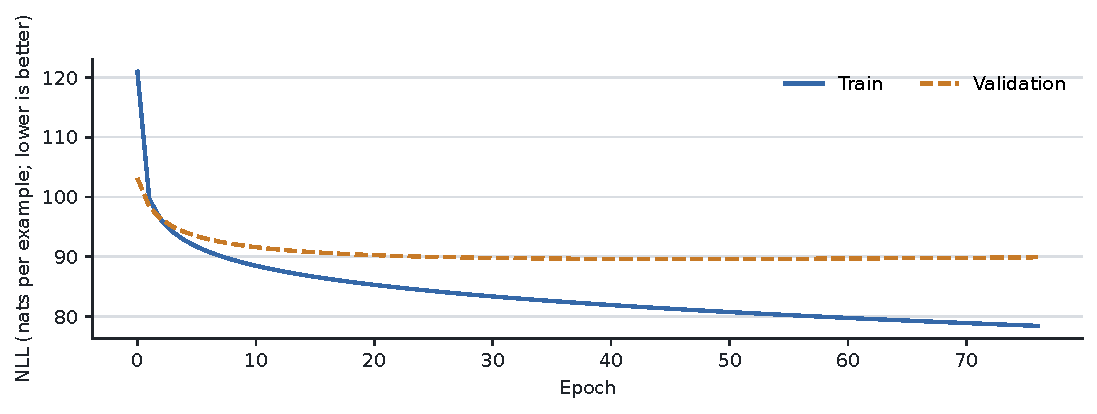
\includegraphics[width=0.72\textwidth]{figures/training_validation.pdf}
\caption{Reconstruction training and validation NLL. Validation NLL is minimized
at epoch index 46 (89.613 nats); training stops after index 76.}
\label{fig:reconstruction-training}
\end{figure}

\section{Reconstruction result}
The selected checkpoint reaches 88.769 test nats, an absolute difference of
0.369 nats (0.42\%) from the paper's central result and inside its interval
$[87.95,88.85]$. Figure~\ref{fig:reconstruction-samples} shows ancestral samples.

\begin{figure}[H]
\centering
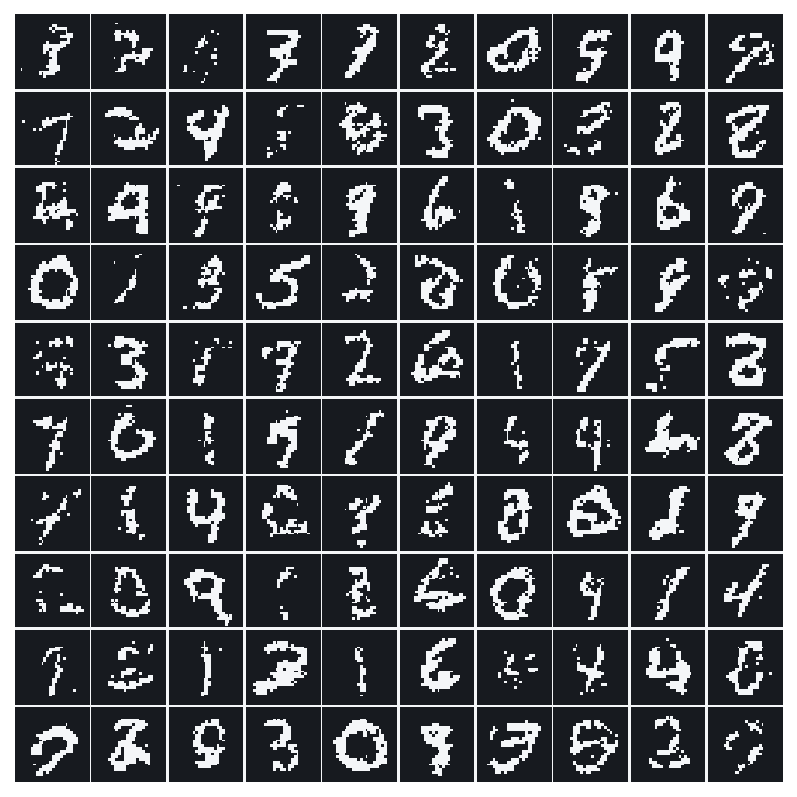
\includegraphics[width=0.29\textwidth]{figures/mnist_samples.pdf}
\caption{One hundred ancestral samples from reconstructed MADE (seed 1234).}
\label{fig:reconstruction-samples}
\end{figure}

\part{Architectural Improvement}
\setcounter{section}{0}

\section{Spatial masked-convolution architecture}
Dense MADE ignores the known $28\times28$ geometry. We therefore replace the
dense hidden transformation with a compact PixelCNN-style decoder
\citep{oord2016pixelcnn}: a strict type-A $7\times7$ masked input convolution,
four type-B $3\times3$ masked residual blocks with 32 channels, and a $1\times1$
output projection. A strict masked linear path supplies global dependence on
earlier pixels. The architecture uses a fixed raster ordering and 653,281
parameters. For residual block $r$,
\begin{align}
h_0 &= \operatorname{ReLU}(\operatorname{Conv}_{A}(x)),\\
h_{r+1} &= \operatorname{ReLU}\!\left(h_r+\operatorname{Conv}_{B,r}(h_r)\right),\\
a(x) &= \operatorname{Conv}_{1\times1}(h_4)+(D\odot M_D)x.
\end{align}
Type A excludes the current pixel; type B includes the current hidden location
but cannot introduce access to the current input. Automatic-Jacobian tests
confirm zero derivative from every logit to itself and all future pixels. The
dataset, Bernoulli NLL, optimizer, batch size, seed, and checkpoint rule remain
unchanged.

\section{Training and improved result}
Figure~\ref{fig:pixelcnn-training} shows the complete 100-epoch trajectory. The
best validation value occurs at the final checkpoint, where the full test NLL is
87.399 nats. This is 1.370 nats below the reconstruction and 1.001 nats below
the paper's central value. It corresponds to 1.98 fewer ideal coding bits per
image and about $e^{1.370}=3.94$ times greater geometric-mean test probability.

\begin{figure}[H]
\centering
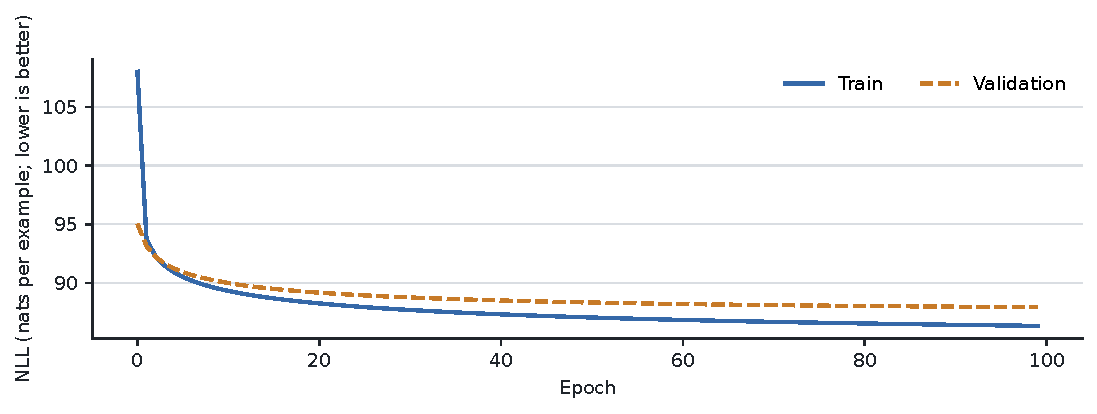
\includegraphics[width=0.72\textwidth]{figures/pixelcnn_training_validation.pdf}
\caption{PixelCNN training and validation NLL across the initial five epochs and
the resumed run through epoch index 99.}
\label{fig:pixelcnn-training}
\end{figure}

\begin{figure}[H]
\centering
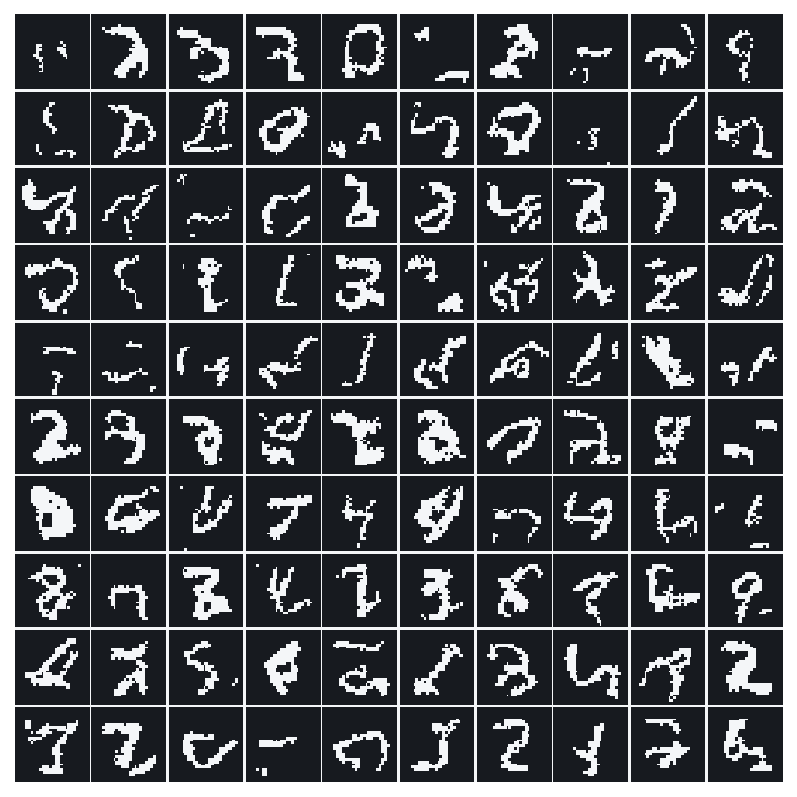
\includegraphics[width=0.29\textwidth]{figures/pixelcnn_samples.pdf}
\caption{One hundred ancestral samples from the improved checkpoint (seed 1234).}
\label{fig:pixelcnn-samples}
\end{figure}

\part{Summary}
\setcounter{section}{0}

\section{Common evaluation standard}
Every reconstructed checkpoint is selected by validation NLL and evaluated once
on the complete 10,000-example test split. The course sample metric is unbiased
squared MMD with the prespecified kernel
$k(x,y)=\exp[-\lVert x-y\rVert_2^2/(2\cdot196)]$. Both models use the same first
100 held-out vectors and 100 ancestral samples generated with seed 1234. Runtime
is end-to-end training wall time, and parameter counts include all trainable
weights and biases.

\section{Three-way comparison}
\begin{table}[H]
\centering
\caption{Selected paper condition, reconstruction, and improved-model results.
Lower is better for NLL and MMD.}
\label{tab:three-way}
\begin{tabular}{@{}lrrr@{}}
\toprule
Metric & Selected paper condition & Reconstruction & Improved PixelCNN \\
\midrule
Test NLL (nats) & $88.40\pm0.45$ & 88.769 & \textbf{87.399} \\
Unbiased MMD$^2$ & --- & \textbf{0.06497} & 0.06836 \\
Trainable parameters & 12,552,784 & 12,552,784 & \textbf{653,281} \\
Training wall time & not reported & $\sim$8m 31s & 14m 53s \\
Selected epoch & not reported & 47 & 100 \\
Autoregressive ordering & fixed shuffled & fixed shuffled & fixed raster \\
\bottomrule
\end{tabular}
\end{table}

\section{Discussion}
The spatial architecture produces a material likelihood gain while reducing
parameter count by 94.8\%, but native convolutional computation takes longer
than the wide dense baseline. MMD$^2$ is slightly worse, so the likelihood gain
does not imply a uniform sample-quality improvement under this finite-sample
kernel test. A direct masked path improved NLL only marginally;
degree-preserving residual and dense-bottleneck MADE variants did not justify
full adoption. The successful result came from matching the architecture to
image geometry while preserving exact autoregressive likelihood evaluation.
The improved model outperforms the selected compute-feasible condition, but its
87.399 nats does not surpass the paper's larger two-layer, 32-mask result of
$86.64\pm0.44$. One seed establishes the controlled result but not cross-seed
statistical significance.

\clearpage
\begingroup
\small
\setlength{\bibsep}{3pt}
\bibliographystyle{plainnat}
\bibliography{references}
\endgroup

\end{document}
